% ============================================================
%  Mattia Pagetti — CV
%  Retro-futurist one-pager. Built with Tectonic (XeTeX):
%    make cv            → public/CV_2026.pdf  (no phone/address/DOB)
%    make cv-private    → cv/build/CV_2026_private.pdf (full contact details)
%  Do not \input this file directly: use CV_2026.tex / CV_2026_private.tex,
%  which set \ifprivate before loading it.
% ============================================================
\documentclass[10pt,a4paper]{article}

\ifprivate\def\bandH{4.65}\else\def\bandH{4.25}\fi
\usepackage[a4paper,left=1.35cm,right=1.35cm,top=\dimexpr\bandH cm+0.7cm\relax,bottom=0.9cm]{geometry}
\usepackage{fontspec}
\usepackage{xcolor}
\usepackage{graphicx}
\usepackage{tikz}
\usetikzlibrary{calc}
\usepackage[most]{tcolorbox}
\usepackage{enumitem}
\usepackage{fontawesome5}
\usepackage[hidelinks]{hyperref}
\usepackage{microtype}
\usepackage{amssymb}

\graphicspath{{assets/}{../public/logos/}}
\pagestyle{empty}
\setlength{\parindent}{0pt}

% ---------- type -------------------------------------------------
\setmainfont{FiraSans}[Extension=.otf,UprightFont=*-Light,BoldFont=*-Medium,
  ItalicFont=*-LightItalic,BoldItalicFont=*-MediumItalic]
\newfontfamily\adv{texgyreadventor}[Extension=.otf,UprightFont=*-regular,BoldFont=*-bold]
\newfontfamily\mono{FiraMono}[Extension=.otf,UprightFont=*-Regular,BoldFont=*-Medium]

% ---------- palette (shared with the website) --------------------
\definecolor{lunar}{HTML}{16202B}    % night sky
\definecolor{lunarsoft}{HTML}{2B3A4A}
\definecolor{cream}{HTML}{F4EDE1}    % paper
\definecolor{orange}{HTML}{D9622B}   % lounge-lamp orange
\definecolor{mustard}{HTML}{E3A72F}
\definecolor{teal}{HTML}{2E6B73}
\definecolor{ink}{HTML}{1E1E1E}
\definecolor{mute}{HTML}{5B5F66}
\color{ink}

% ---------- helpers ----------------------------------------------
\newcommand{\kw}[1]{\textbf{\color{lunar}#1}}
\newcommand{\spaced}[2]{{\addfontfeatures{LetterSpace=#1}#2}}

\newcommand{\cvsection}[2]{%
  \vspace{2pt}%
  {\mono\fontsize{7}{8}\selectfont\color{orange}#1}\hspace{5pt}%
  {\adv\bfseries\fontsize{12.5}{14}\selectfont\color{lunar}\spaced{8}{\MakeUppercase{#2}}}%
  \hspace{6pt}{\color{lunar}\leaders\hrule height 0.6pt\hfill}\kern0pt
  \par\vspace{7pt}}

% Experience timeline entry: #1 filled? (true/false) #2 logo #3 title
% #4 company #5 dates #6 place, body = bullets
\newtcolorbox{tlentry}[1]{enhanced,blank,left=13pt,top=0pt,bottom=11pt,
  borderline west={0.7pt}{3.2pt}{lunar!35},
  overlay={%
    \ifx#1t%
      \fill[orange] ([xshift=3.55pt,yshift=-5.5pt]frame.north west) circle (3.2pt);
    \else
      \fill[cream] ([xshift=3.55pt,yshift=-5.5pt]frame.north west) circle (3.2pt);
      \draw[lunar,line width=0.8pt] ([xshift=3.55pt,yshift=-5.5pt]frame.north west) circle (2.8pt);
    \fi}}

\newcommand{\entryhead}[5]{%
  {\raisebox{-1.5pt}{\includegraphics[height=10pt]{#1}}\hspace{4pt}%
   \adv\bfseries\fontsize{10.5}{12}\selectfont\color{lunar}#2}\par\vspace{1pt}
  {\bfseries\color{orange}#3}\hfill
  {\mono\fontsize{7.5}{9}\selectfont\color{mute}#4\hspace{6pt}\textbar\hspace{6pt}#5}\par
  \vspace{2pt}}

\setlist[itemize]{leftmargin=9pt,labelsep=4pt,itemsep=3.2pt,topsep=2pt,parsep=0pt,before=\raggedright\fontsize{9.4}{12.2}\selectfont,
  label={\color{orange}\scriptsize\raisebox{1pt}{$\blacktriangleright$}}}

\newtcbox{\chip}{on line,enhanced,boxrule=0.5pt,arc=1.6pt,
  colback=cream,colframe=lunar!70,left=2.6pt,right=2.6pt,top=1.1pt,bottom=1.1pt,
  fontupper=\mono\fontsize{7.2}{8}\selectfont\color{lunar}}

\newcommand{\skillgroup}[2]{%
  {\adv\bfseries\fontsize{8.5}{10}\selectfont\color{teal}\spaced{4}{\MakeUppercase{#1}}}\par
  \vspace{3pt}{\raggedright\linespread{1.55}\selectfont #2\par}\vspace{6pt}}

\newcommand{\contact}[2]{{\color{mustard}#1}\hspace{3.5pt}#2}

% ============================================================
\begin{document}

% ---------- header band (absolute) -------------------------------
\begin{tikzpicture}[remember picture,overlay]
  \coordinate (B) at ($(current page.north west)+(0,-\bandH cm)$);
  \fill[lunar] (current page.north west) rectangle ($(current page.north east)+(0,-\bandH cm)$);
  % stars
  \foreach \x/\y/\r in {11.2/-0.6/0.5,12.3/-1.4/0.35,13.1/-0.45/0.6,14.6/-1.0/0.4,
                        10.4/-1.9/0.35,15.9/-0.7/0.5,17.6/-1.3/0.35,19.2/-0.5/0.45,
                        18.3/-3.2/0.35,9.6/-0.4/0.3,16.8/-3.5/0.4,12.8/-3.3/0.3}
    \fill[cream!85] ($(current page.north west)+(\x,\y)$) circle (\r pt);
  % orbits around the portrait
  \coordinate (P) at ($(current page.north east)+(-3.05cm,-2.25cm)$);
  \draw[lunarsoft,line width=0.6pt,rotate around={-14:(P)}] (P) ellipse (3.6cm and 0.95cm);
  \draw[lunarsoft,line width=0.6pt,rotate around={-14:(P)}] (P) ellipse (2.6cm and 0.62cm);
  \fill[mustard] ($(P)+(-3.35cm,0.95cm)$) circle (2.1pt);
  \fill[orange]  ($(P)+(2.15cm,-0.85cm)$) circle (1.6pt);
  % 70s triple stripe
  \fill[mustard] (B) rectangle ($(B)+(\paperwidth,-0.11cm)$);
  \fill[orange]  ($(B)+(0,-0.14cm)$) rectangle ($(B)+(\paperwidth,-0.25cm)$);
  \fill[teal]    ($(B)+(0,-0.28cm)$) rectangle ($(B)+(\paperwidth,-0.39cm)$);
  % portrait
  \begin{scope}
    \clip (P) circle (1.55cm);
    \node at (P) {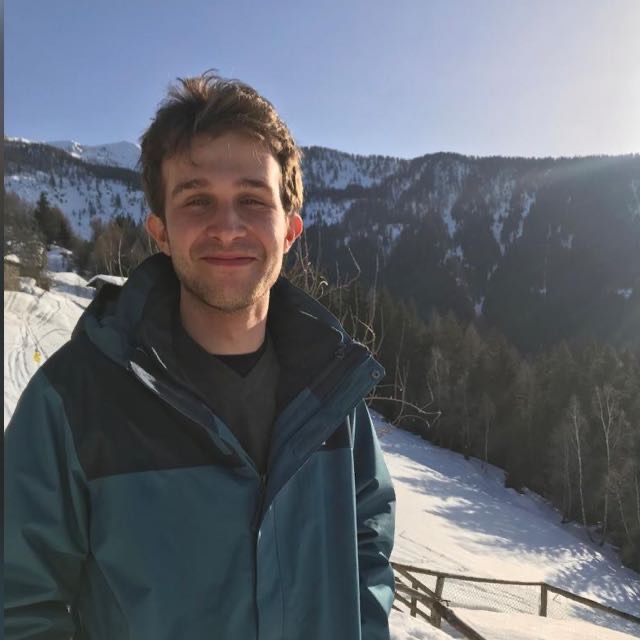
\includegraphics[width=3.15cm]{photo.png}};
  \end{scope}
  \draw[mustard,line width=2.2pt] (P) circle (1.55cm);
  \draw[cream,line width=0.5pt] (P) circle (1.72cm);

  % identity
  \node[anchor=north west,inner sep=0pt,text width=13.3cm,align=left]
    at ($(current page.north west)+(1.35cm,-0.82cm)$) {%
    {\mono\fontsize{7.5}{9}\selectfont\color{orange}\spaced{20}{// CURRICULUM VITAE · 2026}}\\[5pt]
    {\adv\bfseries\fontsize{30}{32}\selectfont\color{cream}\spaced{4}{MATTIA}\hspace{0.32em}\spaced{4}{PAGETTI}}\\[4pt]
    {\adv\fontsize{12}{14}\selectfont\color{mustard}\spaced{12}{SENIOR DATA ENGINEER}}\\[9pt]
    {\fontsize{8.4}{13}\selectfont\color{cream}%
      \contact{\faEnvelope}{\href{mailto:pagetti.mattia@gmail.com}{pagetti.mattia@gmail.com}}\hspace{11pt}%
      \ifprivate\contact{\faPhone}{+39 331 710 9356}\hspace{11pt}\fi
      \contact{\faLinkedin}{\href{https://linkedin.com/in/mattia-pagetti-40891019b}{mattia-pagetti-40891019b}}\\
      \contact{\faGithub}{\href{https://github.com/Paggio}{github.com/Paggio}}\hspace{11pt}%
      \contact{\faGlobe}{\href{https://paggio.github.io/personal-page/}{paggio.github.io/personal-page}}\hspace{11pt}%
      \ifprivate
        \contact{\faMapMarker*}{Via Tadino 40, Milano (MI)}\\
        \contact{\faStar}{Born in Sondrio (SO), Italy, 21/02/1994}%
      \else
        \contact{\faMapMarker*}{Milano, IT}%
      \fi}};
\end{tikzpicture}%

% ---------- profile ----------------------------------------------
\begin{tcolorbox}[enhanced,blank,borderline west={2pt}{0pt}{orange},left=9pt,top=1pt,bottom=1pt]
{\fontsize{9.8}{13.2}\selectfont\raggedright
Data engineer with six years of building data platforms on \kw{AWS} and \kw{Azure}: from
\kw{Spark}/\kw{Iceberg} lakehouses and \kw{Airflow} pipelines to \kw{Databricks} platforms landed
inside locked-down, multi-account cloud estates. Physics engineer by training, platform engineer
by habit: I like infrastructure that is reproducible, secure by default and pleasant to use.\par}
\end{tcolorbox}
\vspace{11pt}

% ---------- body -------------------------------------------------
\begin{minipage}[t]{0.605\textwidth}
\cvsection{01}{Work Experience}

\begin{tlentry}{t}
\entryhead{nearform_logo.png}{Senior Data Engineer}{Nearform}{03/2026 – now}{Tramore, IE / Milano, IT}
\begin{itemize}
  \item I help clients build modern, scalable \kw{Databricks} platforms with solid CI/CD
        foundations: AI-ready from day one and shipped faster with AI-native developer tooling.
  \item For a UK healthcare provider I designed and built, end to end, a \kw{Databricks on AWS}
        platform in \kw{Terraform}: a customer-managed-VPC workspace per environment on a shared
        \kw{Unity Catalog} metastore, one landing-zone KMS key for all storage and managed
        services, back-end \kw{PrivateLink} and Object-Locked audit logs, all deployed through
        \kw{GitHub Actions} (OIDC, tflint, checkov).
  \item Authored the \kw{AWS Landing Zone Accelerator} changes Databricks needed in a locked-down
        multi-account organisation: scoped RCP exceptions, private VPC endpoints, and closing a
        remediation path that gave cluster nodes a privileged IAM role.
\end{itemize}
\end{tlentry}

\begin{tlentry}{f}
\entryhead{truelayer_logo.png}{Senior Data Engineer $\leftarrow$ Data Engineer}{TrueLayer}{02/2022 – 01/2026}{London, UK / Milano, IT}
\begin{itemize}
  \item Built and ran pipelines aggregating microservice databases, queues, third-party APIs and
        Elasticsearch into S3 (Parquet/\kw{Iceberg}), processed with \kw{Spark} on \kw{EMR},
        queried via Athena and orchestrated by \kw{Airflow} DAGs or \kw{Kubernetes} services.
  \item Promoted to Senior in February 2023, I designed and implemented a new data platform from
        the ground up: automated Aurora snapshots loaded into \kw{Redshift} via \kw{ECS}, \kw{Glue}
        and Step Functions, models in \kw{DBT}, infrastructure in \kw{Terraform}.
\end{itemize}
\end{tlentry}

\begin{tlentry}{f}
\entryhead{illimity_logo.png}{Big Data Engineering Junior Specialist}{Illimity}{05/2020 – 02/2022}{Milano, IT}
\begin{itemize}
  \item Developed and maintained Illimity's data streams on Azure with \kw{Databricks},
        \kw{Data Factory}, \kw{Delta Lake} and \kw{MongoDB}, with all workflows managed through
        Azure DevOps.
\end{itemize}
\end{tlentry}

\begin{tlentry}{f}
\entryhead{max_planck.png}{Doctoral Student}{Max Planck Institute (MPSD)}{09/2019 – 04/2020}{Hamburg, DE}
\begin{itemize}
  \item Theoretical and computational analysis of RIXS cross-sections, running advanced
        simulations of realistic condensed-matter systems.
\end{itemize}
\end{tlentry}
\end{minipage}%
\hfill
\begin{minipage}[t]{0.345\textwidth}
\raggedright
\cvsection{02}{Key Skills}
\skillgroup{Main stack}{\chip{Spark} \chip{Databricks} \chip{Terraform} \chip{Airflow}
  \chip{Iceberg} \chip{DBT} \chip{Kubernetes} \chip{Unity Catalog} \chip{LangGraph} \chip{SDD}}
\skillgroup{AWS}{\chip{Landing Zone (LZA)} \chip{SCP / RCP} \chip{PrivateLink} \chip{KMS}
  \chip{EMR} \chip{Redshift} \chip{Athena} \chip{Glue} \chip{S3} \chip{ECS} \chip{EKS}
  \chip{Lambda} \chip{Step Functions}}
\skillgroup{Azure \& more}{\chip{Data Factory} \chip{Data Lake} \chip{Synapse} \chip{Purview}
  \chip{MongoDB} \chip{RabbitMQ} \chip{GitHub Actions}}

\vspace{2pt}
\cvsection{03}{Education}
{\adv\bfseries\fontsize{9.5}{11}\selectfont\color{lunar}MSc Physics Engineering}\par
{\bfseries\color{orange}Politecnico di Milano}\hfill{\mono\fontsize{7.5}{9}\selectfont\color{mute}02/2017 – 04/2019}\par
\vspace{1pt}{\fontsize{8.6}{10.5}\selectfont Nanophysics \& Nanotechnology\\Grade 108/110}\par
\vspace{7pt}
{\adv\bfseries\fontsize{9.5}{11}\selectfont\color{lunar}BSc Physics Engineering}\par
{\bfseries\color{orange}Politecnico di Milano}\hfill{\mono\fontsize{7.5}{9}\selectfont\color{mute}10/2013 – 02/2017}\par
\vspace{1pt}{\fontsize{8.6}{10.5}\selectfont Grade 91/110}\par

\vspace{9pt}
\cvsection{04}{Publications}
{\fontsize{8.8}{11}\selectfont\bfseries\color{lunar}Determining the Electron-Phonon Coupling in
Superconducting Cuprates by Resonant Inelastic X-ray Scattering: Methods and Results on
Nd\textsubscript{1+x}Ba\textsubscript{2−x}Cu\textsubscript{3}O\textsubscript{7−δ}}\par
\vspace{2pt}
{\bfseries\color{orange}Politecnico di Milano}\hfill{\mono\fontsize{7.5}{9}\selectfont\color{mute}2019}\par
\vspace{1pt}
{\raggedright\fontsize{8.6}{10.5}\selectfont The actual role of electron-phonon coupling in high-T\textsubscript{c}
superconductors, investigated. \href{https://arxiv.org/abs/1906.01270}{\color{teal}\mono\fontsize{7.5}{9}\selectfont arXiv:1906.01270 \faExternalLink*}}\par
\end{minipage}

\vfill
{\centering\mono\fontsize{6.5}{8}\selectfont\color{mute}\spaced{30}{THANK YOU FOR STAYING · PLEASE RETURN YOUR KEY AT RECEPTION}\par}
\end{document}
